\begin{figure}[!h]
  \centering
  \caption{Results on stationarity test comparing average grade across years}
  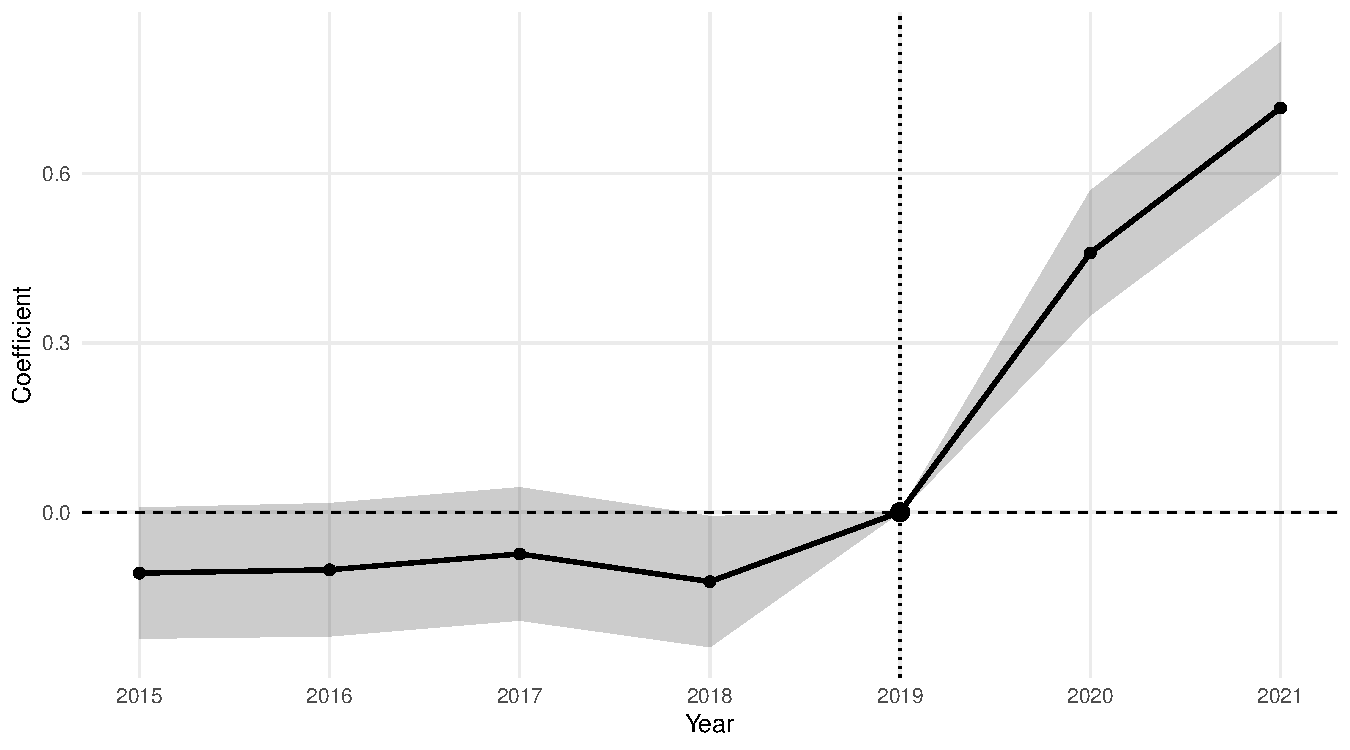
\includegraphics[width=\textwidth]{figures/Empirical_Model/event_study_plot.pdf}
  \label{fig:event_study}
  \vspace{0.5ex}
  \caption*{\footnotesize Note: The figure displays the exam level year-to-year differences in probability to receive a top grade (A or $\text{A}^*$) between the reference year (2019) and other years from 2015 to 2021. The sample is the universe of A-level exams used for admissions at British universities through the centralized administrative system (N = 2,802,651). Year-specific coefficients and 95\% confidence intervals are from a logistic regression that regresses a success dummy indicating the student receiving a top grade (A or $\text{A}^*$) on a series of time indicator dummy variables while controlling for students' achievement score in a previous standardized national exam (GCSE) in mandatory subjects (mathematics and English literature) and a dummy variable for the subject course of the exam.. Standard errors are clustered at the school-subject course level. }
\end{figure}



\begin{figure}[!htbp]
    \centering
    \caption{Stationatity test by (a) school types  and (b) parental occupation class}
    \begin{subfigure}[t]{\linewidth}
        \centering
        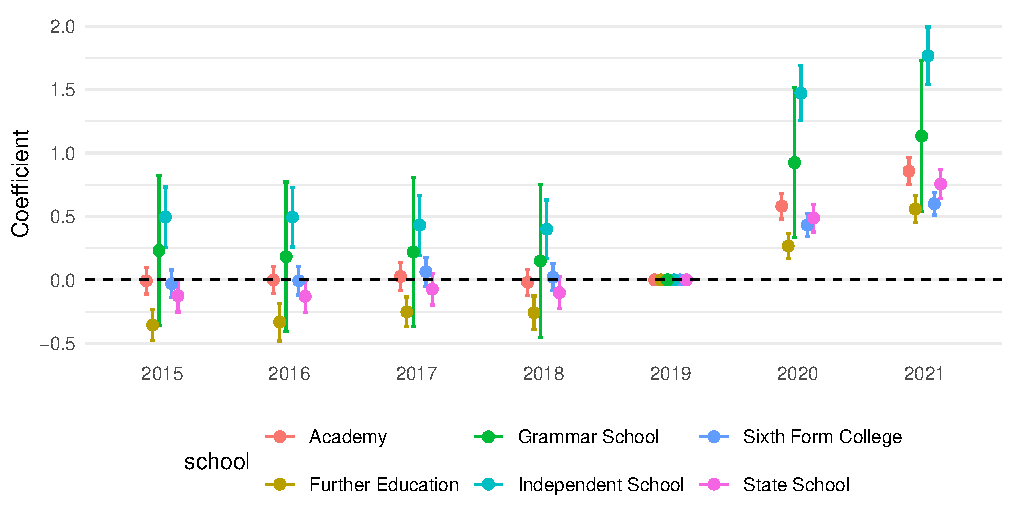
\includegraphics[width = \textwidth]{figures/Empirical_Model/BySchoolType.pdf}
        \label{fig:event_study_type}
        \end{subfigure}

      \vspace{4pt} % small gap between panels
    
    \begin{subfigure}[t]{\linewidth}
        \centering
        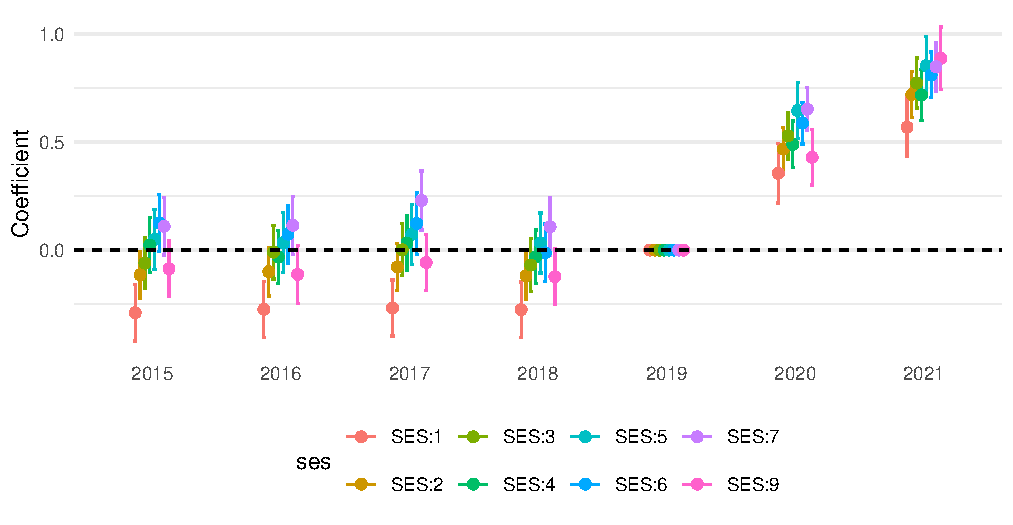
\includegraphics[width = \textwidth]{figures/Empirical_Model/BySES.pdf}
        \label{fig:event_study_type}
    \end{subfigure}
    \label{fig:inflation_subjects_20_21}
    \vspace{-0.5em}
    \caption*{\footnotesize Note: The figure displays the exam level year-to-year differences in probability to receive a top grade (A or $\text{A}^*$) between the reference year (2019) and other years from 2015 to 2021 after sub-sampling the sample by the test takers' (a) school types or (b) parents' parental occupation class. The sample is the universe of A-level exams used for admissions at British universities through the centralized administrative system (N = 2,802,651). Year-specific coefficients and 95\% confidence intervals are from a logistic regression that regresses a success dummy indicating the student receiving a top grade (A or $\text{A}^*$) on a series of time indicator dummy variables while controlling for students' achievement score in a previous standardized national exam (GCSE) in mandatory subjects (mathematics and English literature) and a dummy variable for the subject course of the exam. Coefficients are estimated jointly by interacting the times indicator dummy with either a (a) school type indicator or a (b) parental occupation indicator. Standard errors are clustered at the school-subject course level. }
\end{figure}
\clearpage
